\documentclass[11pt,letterpaper,twoside,english]{article}

\usepackage[margin=1.4in]{geometry} % controls the size of the margins

% Special symbols, etc.
\usepackage{amssymb,amsbsy,latexsym,ytableau}
\usepackage{amsmath}
\usepackage{graphics, subfigure, float} 
\usepackage{cancel}
%\usepackage{todonotes}
% Encoding settings
\usepackage[latin1]{inputenc}
\usepackage[american]{babel}
\usepackage[T1]{fontenc} 
\usepackage{tikz}

\usepackage{titling} % allows posttitle command

% AMS Math packages

\usepackage{amscd,amsthm}

\usepackage{verbatim, comment} % can comment out text 
\usepackage{mdwlist} 

% Graphics
%\usepackage[dvips]{graphicx,epsfig,color}
%\usepackage{subfigure}
%\usepackage{pst-all}
%\usepackage{pstricks-add}
\usepackage{hyperref}  % can only be used with pdflatex - gives hyperlinks
\usepackage{bm} % bold math font
\usepackage{bbm}

\usepackage{todonotes}

\newtheoremstyle{theorem}{1em}{1em}{\slshape}{0pt}{\bfseries}{.}{ }{}
\theoremstyle{theorem}
\newtheorem{theorem}{Theorem}[section]
\newtheorem*{theorem*}{Theorem}
\newtheorem{corollary}[theorem]{Corollary}
\newtheorem{proposition}[theorem]{Proposition}
\newtheorem{lemma}[theorem]{Lemma}
\newtheorem{claim}[theorem]{Claim}
\newtheorem{conjecture}[theorem]{Conjecture}
\newtheorem{definition}[theorem]{Definition}
\newtheorem*{claim*}{Claim}

\theoremstyle{remark}
\newtheorem{remark}[theorem]{Remark}
\newtheorem*{remark*}{Remark}
\newtheorem{algorithm}{Algorithm}
\newtheorem*{question*}{Question}
\newtheorem{question}{Question}
\newtheorem{example}[theorem]{Example}

\providecommand{\setN}{\mathbb{N}}
\providecommand{\setZ}{\mathbb{Z}}
\providecommand{\setQ}{\mathbb{Q}}
\providecommand{\setR}{\mathbb{R}}
\providecommand{\E}{\mathrm{E}}
\providecommand{\Pr}{\mathrm{Pr}}
\providecommand{\Var}{\mathrm{Var}}

\tikzset
{
    treenode/.style = {circle, draw=black, align=center, minimum size=1cm},
}

\makeatother

\title{Almost Orthogonal vectors} 

\author{Yajit Jain, Deepak Narayanan, Leon Zhang}

\begin{document}

\maketitle

\section{Introduction}
Given a dimension $n$ and a number $N > n$ of vectors, we want to find vectors $v_1, v_2, \ldots, v_N \in \mathbb{R}^n$ of unit length, such that
$$\epsilon = \max_{i \neq j} \{ |v_i \cdot v_j|^2 \}$$
is as small as possible.

\section{$n=2$, generic $N$}
In this section, we consider the problem of almost orthogonal vectors of dimensionality $2$.

It is obvious that for $N=2$, we can find an $\epsilon$ equal to $0$, since it easy to pick two unit vectors $v_1$ and $v_2$ of unit length that are orthogonal to each other -- a simple example of such vectors is $[1, 0]^T$ and $[0, 1]^T$. 

However, we see that the problem gets harder for larger $N$. Let us first consider the specific case of $N=3$; once we build some intuition for the problem, we will try to generalize to generic $N$.
\\

It's clear that when $N=3$, the value of $\epsilon$ must be greater than $0$, since there is no way three dimensionality-$2$ vectors can be orthogonal to each other.

In addition, we see that for $N=3$, the quantity $\epsilon$ for three unit-length vectors $v_1, v_2, v_3 \in \mathbb{R}^2$ is given by $$\max \{ |v_1 \cdot v_2|^2, |v_1 \cdot v_3|^2, |v_2 \cdot v_3|^2 \}$$

Since we don't care about the sign of the dot product between any two vectors, if we define the unit vectors $v_4, v_5, v_6 \in \mathbb{R}^2$ to be the reverses of $v_1, v_2, v_3$ respectively, then we see that $\epsilon$ can be equivalently expressed as $$\max_{i \neq j} \{|v_i \cdot v_j |^2 \}$$
where $i, j \in \{1,2,\ldots,6\}$ -- the above result holds because if the vector $\mathcal{R}(v)$ is the reverse of the vector $v$, then $|v \cdot v'| = |\mathcal{R}(v) \cdot v'|$ for some arbitrary vector $v'$.

Without loss of generality, let $x_1 = [1, 0]^T$; then since $x_4$ is the reverse of $x_1$, we see that $x_4 = [-1, 0]^T$. Also, without loss of generality assume that $x_2$ and $x_3$ are above the $x$-axis, and that $x_2$ is to the right of $x_3$.

\begin{figure}
    \centering
    \begin{tikzpicture}[yscale=-1] 
        % x-axis
        \draw [thick,->] (-4.5, 0) -- (4.5, 0);
        % y-axis
        \draw [thick,->] (0, 4.5) -- (0, -4.5);
        % origin label
        \node at (-0.5, 0.3) {\text{$(0, 0)$}};
        % x-axis label
        \node at (4.5, 0.5) {\text{$x$}};
        % y-axis label
        \node at (0, -5) {\text{$y$}};
        % circle
        \draw (0,0) circle (3cm);
        \draw (3,0)[blue,fill=blue] circle (0.1cm);
        \draw (1.5, -2.59)[blue,fill=blue] circle (0.1cm);
        \draw (-1.5, -2.59)[blue,fill=blue] circle (0.1cm);
        
        \draw [thick,-,blue] (3, 0) -- (0, 0);
        \draw [thick,-,blue] (1.5, -2.59) -- (0, 0);
        \draw [thick,-,blue] (-1.5, -2.59) -- (0, 0);
        
        \node at (4, -0.3) {\text{$x_1 = [1,0]$}};
        \node at (2.8, -3.1) {\text{$x_2 = [\cos \pi/3,\sin \pi/3]$}};
        \node at (-2.8, -3.1) {\text{$x_3 = [\cos 2\pi/3,\sin 2\pi/3]$}};
    \end{tikzpicture}
    \caption{A configuration of three unit vectors that produce the optimum $\epsilon$ for $n=2, N=3$}
\end{figure}


Let $\theta_1$ be the angle between $x_1$ and $x_2$, $\theta_2$ be the angle between $x_2$ and $x_3$ and $\theta_3$ be the angle between $x_3$ and $x_4$. Now, it is easy to see that $\theta_1 + \theta_2 + \theta_3 = \pi$ and that $$\epsilon = \max_{i \in \{1,2,3\}} \cos ^2 \theta_i$$

Before proceeding, we state and prove the following lemma.
\begin{lemma}
Consider $n$ angles $\theta_1, \theta_2, \ldots, \theta_n \in [0, \pi]$ s.t. $\theta_1 + \theta_2 + \ldots + \theta_n = \pi$. Then $\epsilon = \max_i \cos^2 \theta_i$ must equal $\cos^2 \theta_j$ where $j = \text{argmin }\theta_i$.
\end{lemma}

\begin{proof}

Our arguments will hinge on the fact that for all $\theta \in [0, \pi/2]$, the function $\cos \theta$ is decreasing. Without loss of generality, let us assume that $\theta_1 \geq \theta_2 \geq \ldots \theta_n$. Hence we want to prove that $\epsilon$ is equal to $\cos^2 \theta_n$.

We split our proof into two cases,
\begin{itemize}
\item $\theta_1, \theta_2, \ldots, \theta_n \in [0, \pi/2]$: This is easy to see from the fact that $\cos \theta$ is a decreasing function in $\theta$ if $\theta \in [0, \pi/2]$.

\item One of $\theta_1, \theta_2, \dots, \theta_n$ is greater than $\pi/2$:
\begin{figure}
    \centering
    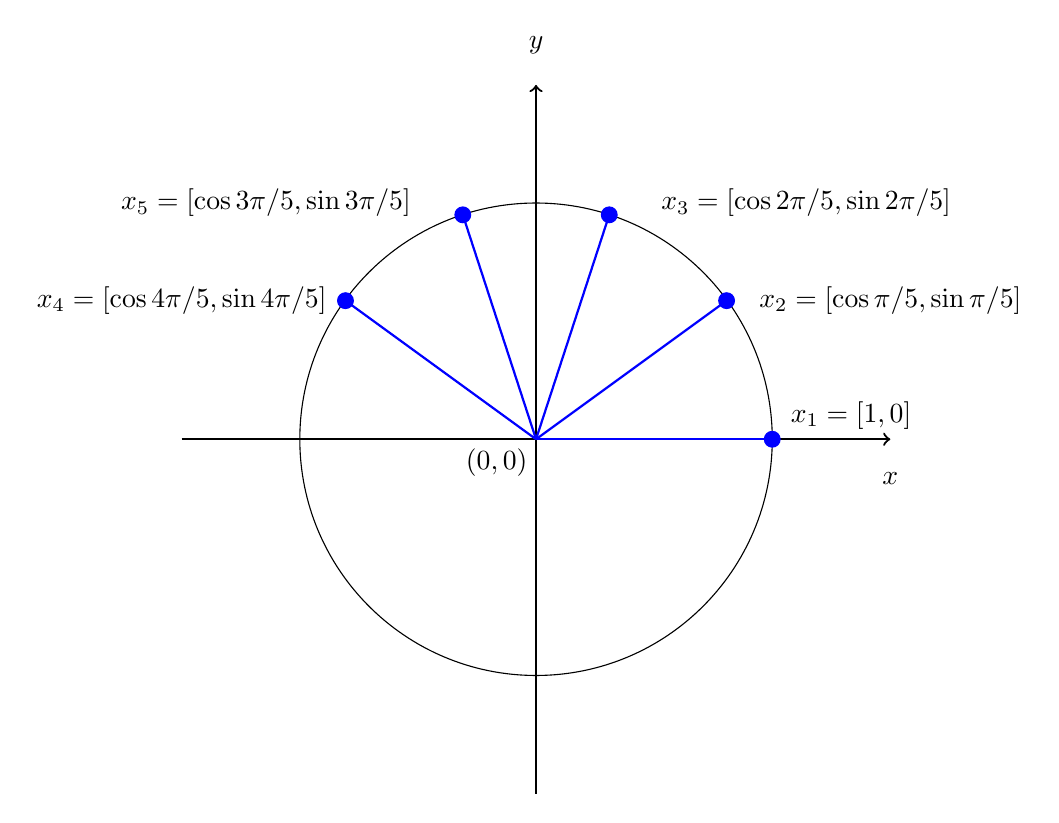
\begin{tikzpicture}[yscale=-1] 
        % x-axis
        \draw [thick,->] (-4.5, 0) -- (4.5, 0);
        % y-axis
        \draw [thick,->] (0, 4.5) -- (0, -4.5);
        % origin label
        \node at (-0.5, 0.3) {\text{$(0, 0)$}};
        % x-axis label
        \node at (4.5, 0.5) {\text{$x$}};
        % y-axis label
        \node at (0, -5) {\text{$y$}};
        % circle
        \draw (0,0) circle (3cm);
        \draw (3,0)[blue,fill=blue] circle (0.1cm);
        \draw (2.42, -1.76)[blue,fill=blue] circle (0.1cm);
        \draw (0.93, -2.85)[blue,fill=blue] circle (0.1cm);
        \draw (-2.42, -1.76)[blue,fill=blue] circle (0.1cm);
        \draw (-0.93, -2.85)[blue,fill=blue] circle (0.1cm);
        
        \draw [thick,-,blue] (3, 0) -- (0, 0);
        \draw [thick,-,blue] (2.42, -1.76) -- (0, 0);
        \draw [thick,-,blue] (0.93, -2.85) -- (0, 0);
        \draw [thick,-,blue] (-2.42, -1.76) -- (0, 0);
        \draw [thick,-,blue] (-0.93, -2.85) -- (0, 0);
        
        \node at (4, -0.3) {\text{$x_1 = [1,0]$}};
        \node at (4.5, -1.76) {\text{$x_2 = [\cos \pi/5,\sin \pi/5]$}};
        \node at (3.43, -3) {\text{$x_3 = [\cos 2\pi/5,\sin 2\pi/5]$}};
         \node at (-4.5, -1.76) {\text{$x_4 = [\cos 4\pi/5,\sin 4\pi/5]$}};
        \node at (-3.43, -3) {\text{$x_5 = [\cos 3\pi/5,\sin 3\pi/5]$}};
    \end{tikzpicture}
    \caption{A configuration of five unit vectors that produce the optimum $\epsilon$ for $n=2, N=5$}
\end{figure}

Then, if $\theta_1 > \pi/2$ we see that $\cos^2 \theta_1 = \cos^2 (\pi - \theta_1)$ is equal to $\cos^2 (\theta_2 + \theta_3 + \ldots + \theta_n)$. Furthermore, $\pi - \theta_1 = \theta_2 + \theta_3 + \ldots + \theta_n < \pi/2$, which means $\cos^2 \theta_1 = \cos^2 (\theta_2 + \theta_3 + \ldots + \theta_n) < \cos^2 \theta_n$. (since $\theta_n < \theta_2 + \theta_3 + \ldots + \theta_n$)

It is easy to see that for all $i \in \{2, 3, \ldots, n-1\}$, $\cos^2 \theta_i < \cos^2 \theta_n$, from which we can conclude that in this case too, $\epsilon$ is equal to $\cos^2 \theta_n$.

\end{itemize}
\end{proof}

From the above lemma, we can conclude that if $j = \text{argmin } \theta_i$ and $\theta_1 + \theta_2 + \theta_3 = \pi$, then $\epsilon = \cos^2 \theta_j$.

Furthermore, we can obtain an upper bound on $\theta_j$ by observing that $\theta_ 1 + \theta_ 2 + \theta_3 \geq \theta_ j + \theta_j + \theta_j = 3 \theta_j \Rightarrow \theta_j \leq \pi/3$. Since we're interested in the smallest such $\epsilon$ and since the cosine function is a decreasing function in $\theta$ between $0$ and $\pi/2$, we conclude that the optimum value of $\epsilon$ for $n=2$ and $N=3$ is $\cos^2 \pi / 3$. Figure $1$ shows this optimum configuration.

\begin{theorem}
For $n=2$ and arbitrary $N$, the optimum value of $\epsilon$ is given by $\cos^2 \pi/N$.
\end{theorem}

\begin{proof}
The proof is easy to see given the above lemma.

Again without loss of generality, we can assume that the vectors $x_1, x_2, \ldots, x_N$ are on or above the $x$-axis, and that $x_1 = [1,0]^T$ and that $x_{N+1} = [-1,0]^T$.

Let us define $\theta_i$ as the angle between the vectors $x_i$ and $x_{i+1}$. Then, we quickly see that $\theta_1 + \theta_2 + \ldots + \theta_N = \pi$. If $j = \text{argmin } \theta_i$, $\epsilon = \cos^2 \theta_j$.

Since $\theta_ 1 + \theta_2 + \ldots + \theta_N \geq N \cdot \theta_j \Rightarrow \theta_j \leq \pi/N$, we conclude that the optimum $\epsilon$ value is in fact equal to $\cos^2 \pi/N$.
\end{proof}

Figure $2$ shows an optimum configuration for $n=2$ and $N=5$.
\begin{figure}
    \centering
    \begin{tikzpicture}[yscale=-1] 
        % x-axis
        \draw [thick,->] (-4.5, 0) -- (4.5, 0);
        % y-axis
        \draw [thick,->] (0, 4.5) -- (0, -4.5);
        % origin label
        \node at (-0.5, 0.3) {\text{$(0, 0)$}};
        % x-axis label
        \node at (4.5, 0.5) {\text{$x$}};
        % y-axis label
        \node at (0, -5) {\text{$y$}};
        % circle
        \draw (0,0) circle (3cm);
        \draw (3,0)[blue,fill=blue] circle (0.1cm);
        \draw (-1.5, 2.59)[blue,fill=blue] circle (0.1cm);
        \draw (-1.5, -2.59)[blue,fill=blue] circle (0.1cm);
        
        \draw [thick,-,red,dashed] (3, 0) -- (-1.5, 2.59);
        \draw [thick,-,red,dashed] (3, 0) -- (-1.5, -2.59);
        \draw [thick,-,red,dashed] (-1.5, -2.59) -- (-1.5, 2.59);
        
        % \draw [thick,-,blue, dotted] (-3, 0) -- (0, 0);
        % \draw [thick,-,blue, dotted] (1.5, -2.59) -- (0, 0);
        % \draw [thick,-,blue, dotted] (1.5, 2.59) -- (0, 0);
        \draw [thick,-,blue] (3, 0) -- (0, 0);
        \draw [thick,-,blue] (-1.5, 2.59) -- (0, 0);
        \draw [thick,-,blue] (-1.5, -2.59) -- (0, 0);
    \end{tikzpicture}
    \caption{A configuration of three unit vectors that produce the optimum $\epsilon$ for $n=2, N=3$}
\end{figure}

\end{document}